\section{DevOps}
\label{sec:devops}

O termo DevOps tem sido usado com frequência em diversas esferas do
desenvolvimento de software da atualidade, mas por ser um conceito recente
(2008), muita cunfusão ainda é gerada ao tentar definir e trabalhar com
DevOps~\cite{adambertram:2016}. ''A palavra DevOps vem de duas palavras em
inglês, \textit{development} e \textit{operations} (desenvolvimento e operações) e de maneira
geral é a cultura, movimento ou conjunto de práticas que incentiva
a comunicação, a colaboração e a integração de desenvolvedores de software
e outros profissionais de TI. Além das práticas também engloba ferramentas
e técnicas que automatizam o processo de entrega de software e as mudanças
de infraestrutura~\cite{loukides2012devops}~\cite{erich2014mapping}.

Muitas vezes o termo é confundido com uma nova responsabilidade, ou cargo
dentro de uma empresa que desenvolve software, e por mais que seja possível
ter profissionais que tenham proficiência nas ferramentas relacionadas a
DevOps, o ideal, como dito anteriormente, é ter uma melhor comunicação,
colaboração e integração entre os times já existentes. As ferramentas
relacionadas à DevOps facilitam esses aspectos, mas o diferencial é a
mudança no processo de desenvolvimento para absorver essas melhorias
~\cite{adambertram:2016}.

%TODO: parece está faltando mais alguma coisa de DevOps

\section{Métodos Ágeis e DevOps}

A metodologia ágil surgiu como uma resposta às maneiras tradicionais de desenvolvimento
de software considerando uma nova abordagem com relação as práticas, organização,
documentação e foco no desenvolvimento.~\cite{agilemetorg:2016}

Os métodos ágeis são formas de sustentação da filosofia ágil proposta no manifesto
ágil\cite{fowler:2001}. As duas mais populares são o \textit{Scrum} e o \textit{Extreme Programming}. Nelas,
são definidas práticas que eram comumente utilizadas em outros contextos,
mas foram reunidas e adaptadas para se adequarem à filosofia ágil~\cite{shore:2007}.

Diferentemente da metodologia de Cascata, por exemplo, o \textit{Scrum} implementa uma
abordagem iterativa e incremental, podendo assim desenvolver incrementos de
maior valor para o cliente mais cedo, e assim tendo \textit{feedback} para correções
mais frequentes. A Figura~\ref{fig:iterative} mostra um exemplo dessas
Iterações.~\cite{scrumreference:2016}

\begin{figure}[H]
  \centering
  \label{fig:iterative}
  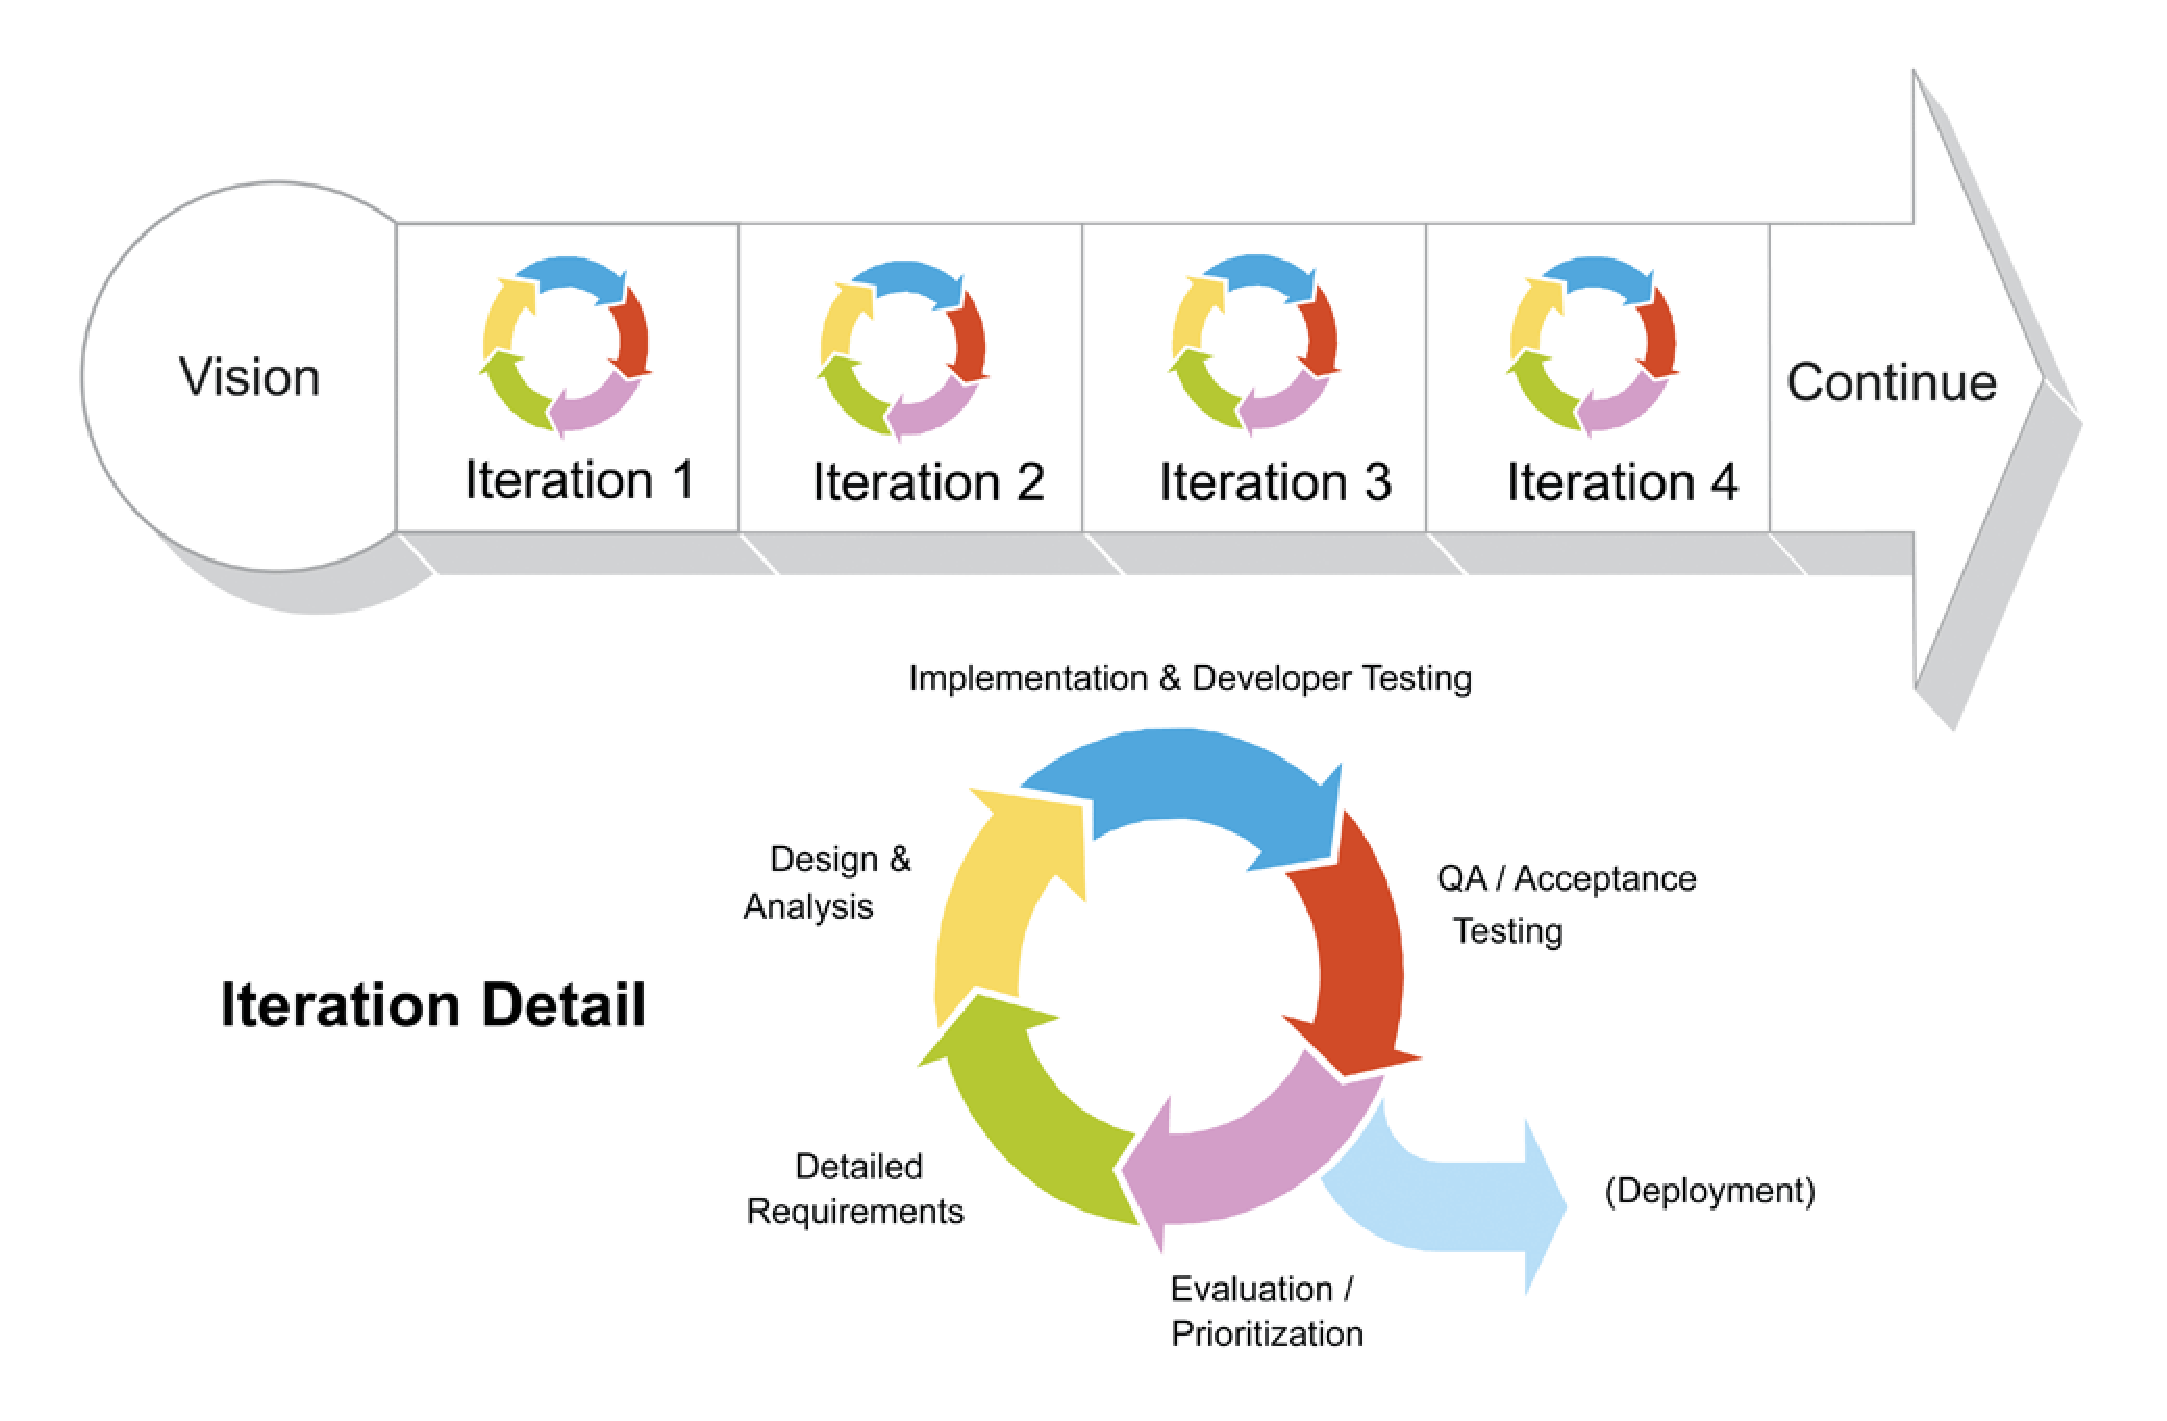
\includegraphics[width=0.8\textwidth]{figuras/iterative.eps}
  \caption{Iterações do Scrum~\cite{scrumreference:2016}.}
\end{figure}

Com a popularização da metodologia de desenvolvimento Ágil, que tem, dentre outros
objetivos, o de entregar com maior frequência, e melhorar a comunicação entre os
times, é simples fazer a relação de DevOps com esse tipo de desenvolvimento.
DevOps nada mais é do que a implementação de conceitos e mudanças organizacionais
e culturais provenientes do pensamento Ágil~\cite{scott2014}.

DevOps tenta alcançar entregas mais frequentes ao preparar um ambiente que facilite,
automatize e integre vários dos processos que antes seriam manuais, e mais
suscetíveis à falhas e atrasos, o que não é possível sem uma equipe integrada
nesse ambiente. Dessa forma, o conceito de entrega contínua e de integração
contínua estão fortemente relacionados à DevOps.~\cite{adambertram:2016}

\subsection{Integração Contínua}

Integração contínua é a prática de integrar diversas partes de um software
desenvolvido em diversas frentes, de maneira periódica, ou a cada mudança.
Foi adotado como parte do método \textit{Extreme Programming} (XP) que sugere integrar
partes do software mais de uma vez por dia \cite{fowler2006continuous}.

Mesmo que não se adote desenvolvimento orientado a teste 
(TDD - \textit{test driven development}), uma funcionalidade só está 
pronta se estiver com seus testes implementados, levando em consideração 
metodologias de desenvolvimento Ágil. E, dessa forma, a integração 
contínua pode dar retorno com relação aos resultados desses testes a todo momento que ocorrer uma nova integração do software. %TODO: referencia

\subsection{Entrega Contínua}

A Entrega Contínua é uma prática adotada pelos métodos ágeis que tem o objetivo
de preparar um \textit{software} para que ele seja passível de ser posto em produção a
qualquer momento~\cite{olausson:2016}. 

A prática de Entrega Contínua  é frequentemente confundida com a Integração
Contínua. Existe uma relação de dependência entre as duas práticas para
construir uma estrutura que possa sustentar a entrega contínua de um
\textit{software}.~\citeonline{olausson:2016} resumem os dois em:

\begin{itemize}
  \item \textbf{Integração Contínua}: é voltada para estabelecer uma rápida
    validação da fase de desenvolvimento;
  \item \textbf{Entrega Contínua}: é voltada para estabelecer uma cultura onde
    pode-se oferecer um recurso ou \textit{feature} para o cliente a qualquer
    momento.
\end{itemize}

